%!Mode::"TeX:UTF-8"

\documentclass[12pt, a4paper]{book}

\usepackage{CJKutf8}
\usepackage[unicode={true}]{hyperref}
\usepackage{color}
\usepackage{graphicx}

\title{\textbf{The Legendary Romance of Seven Hulus}}
\author{Executive Cabinet of Xiao-Ming Kingdom}
%\date{}

\begin{document}
\begin{CJK}{UTF8}{gbsn}

    \maketitle
    \clearpage
    \thispagestyle{empty}

    \frontmatter
    
    \vspace*{50 mm}
    \begin{center}
    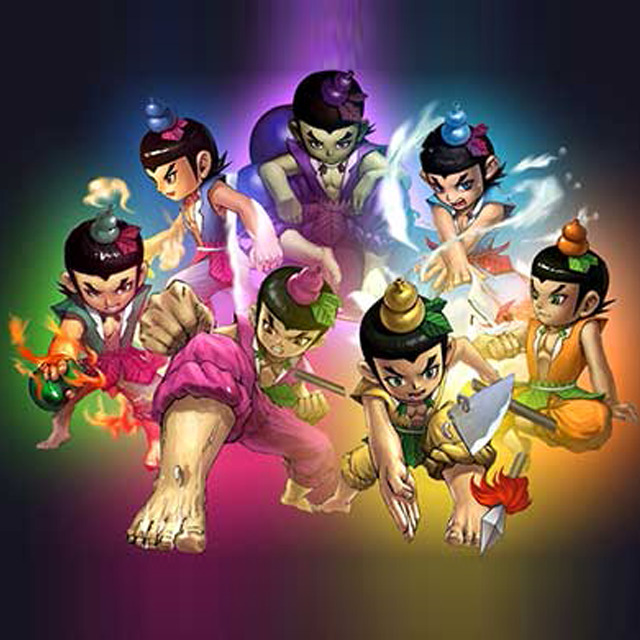
\includegraphics[width=0.6\textwidth]{figure/hulu.png}
    \end{center}

    %\include{preface/intro}
    %!Mode::"TeX:UTF-8"

\chapter{Preface}

谨以此纪念孙晓峰葫芦娃断浆行舟的昂扬青春。

    \chapter{Acknowledgement}

谨对小明王朝执行内阁全体成员为本书提供的宝贵史料致以诚挚的谢意。


    \chapter{楔子  穿山甲误走蛇蝎怪 盘古氏结缘葫芦藤}
    
    \tableofcontents

    \mainmatter

    %%!Mode::"TeX:UTF-8"

\chapter[历酷暑四字建班号 流火季七葫聚帝都]{历酷暑四字建班号\\\quad流火季七葫聚帝都}

没内容,你咬我啊

    %\chapter[着绿装众娃皆做火 披迷彩夜探北沙窝]{着绿装众娃皆做火\\\quad披迷彩夜探北沙窝}

没内容,你咬我啊


    \chapter{武曲星再起关中地 赤葫芦伟力撼京营}
    
    没内容就是没内容。

    \chapter{修杨树辽东王出世 上镜头橙葫芦初名}
    
    没内容你咬我啊。
    
    \chapter{关外雪冻碎钢筋骨 关内风吹干黄葫芦}

    \chapter{军训场佳偶初相会 火葫芦观星撩良辰}

    \chapter{强迫症病发残足趾 水葫芦玩火焚自身}

    \chapter{浪里白条萌相毕露 行踪无影蓝娃狐行}

    \chapter{盘天象处女拱红日 收万物紫娃覆雨云}

    \chapter{奥运年未及观奥运 流沙河红黄战流沙}

    \chapter{班封零复始新万物 五葫芦聚首紫荆园}

    \chapter{行万里赤葫芦北去 读万卷黄葫芦留燕}

    \chapter{历答辩众葫芦称导 经风雪赤葫芦归京}

    \chapter{四二一七葫芦聚义 东西北众诸侯会师}

    \chapter{带军训蓝娃改送水 管熊宝水娃Angry}

    \chapter{无制服紫娃怒隐身 随拉练三娃摔破膝}

    \chapter{三班倒二娃观八面 一横心大娃战通宵}

    \chapter{军训过再逢一二九 水葫芦灌水强出头}

    \chapter{水娃暴饮水下如牛 火娃添杯火上浇油}
    
    \chapter{建王朝众葫芦组阁 称学士水葫芦秉政}
    
    \chapter{力无穷晋位指挥使 撩良辰职司钦天监}
    
    \chapter{恋百味二娃掌礼部 育后生七娃监国子}
    
    \chapter{悬明镜六娃卿大理 爱唠叨三娃赴六科}
    
    \chapter{秀恩爱少卿出新招 长颈鹿化身大白兔}
    
    \chapter{百色芒果北上帝都 留守葫芦心念二娃}
    
    葫芦三年七月十一日,礼部侍郎娃二八百里速递桂地芒果入京。看守内阁文员,户科给事中娃三收讫,分送驻京阁属,俱喜而歌,以为消暑佳品。
    
    \appendix

    %!Mode::"TeX:UTF-8"

\chapter{七葫大事记}

\begin{itemize}
    \item{2016年7月5日,经小明王朝执行内阁提案,内阁首辅、XX殿大学士袁票拟批蓝,《七葫拍案惊奇》创作计划启动。}
\end{itemize}


\end{CJK}
\end{document}

